\chapter{Scottsdale and the Operating Math of Wealth}

This School of Hard Knocks interview, curated by LazyingArt LLC, behaves like a lecture on wealth mechanics disguised as street access. The host begins with spectacle---luxury cars, whispered tips, a billionaire who owns an NBA team, and a promised meeting with Robert Kiyosaki---but the useful material lies in the ratios and update rules that emerge once people finally talk. No validated mathematical screenshots survived review for this episode, so the diagrams below are transcript-based reconstructions of flow, timing, and scale rather than redrawings of visible board work.

\section{Scottsdale as a Wealth Field}

\paragraph{Anecdote.} The lecture opens with a whispered rumor: there is a billionaire inside, and he owns a basketball team. The host follows the lead immediately and gets an answer almost at once. The Phoenix Suns appear before the formal introduction of the episode; Robert Kiyosaki appears before the long interview with him. The rhythm is deliberate. We are shown the payoff before we are shown the search.

\paragraph{Claim.} Scottsdale is treated as a concentrated field of wealth rather than a random sample of affluent households. Rolls Royce, McLaren, Bentley, valet stands, restaurants, and private entrances are not decorative details. They define the terrain on which the lecture moves.

\paragraph{Mechanism.} The first mechanism is social rather than financial. Wealth may be visible, but information is guarded. The early part of the transcript is full of refusals, brief answers, and people who do not want the camera. The host's first practical rule is therefore this: access has a friction term. In this lecture, repeated approaches are part of the argument, not filler around it.

\section{From Refusal to Real Signal: the FinTech Bottleneck}

\paragraph{Anecdote.} After several rebuffs, the host finally persuades a private founder to speak by proving the legitimacy of the channel. That is an important transition. The first useful doctrine does not come from merely asking harder questions; it comes from making oneself believable enough that a private operator will answer seriously.

\paragraph{Claim.} Once the founder agrees to talk, the host asks the sharpest business question in the first half of the lecture: what blocks the move from a \$10 million company to a \$100 million business? The point is not to learn another origin story. It is to isolate the scale transition itself.

\begin{equation}
S_0 \approx \$10\,\text{million},\qquad S_1 \approx \$100\,\text{million},\qquad \frac{S_1}{S_0} \approx 10.
\end{equation}

We should be careful with notation here. The speaker is not presenting audited accounting categories; he is giving us scale markers. Still, the tenfold jump is the right way to frame the problem.

\paragraph{Mechanism.} The answer is that companies often get in their own way. They address scale only when they must, instead of building process and structure in advance. A clean way to write the thought, though the transcript does not state it algebraically, is

\begin{equation}
\text{stress}_{\text{growth}} \propto \text{demand} - \text{prepared capacity}.
\end{equation}

If prepared capacity lags demand, growth arrives as pressure. If capacity is built early, the firm grows into a shape it has already made room for.

\subsection{Question \& Answer}

\paragraph{Question.} Why do companies choke when they try to scale?

\paragraph{Answer.} Because they confuse growth with reaction. The founder's point is not that growth is mysterious; it is that scale punishes firms that postpone structure until after the shock arrives. The same interview then widens the claim from systems to management. A bad boss becomes instructive precisely because he shows what destroys scale from within: not listening, hiring talent and then silencing it, pushing arbitrary deadlines, and losing sight of customers and employees. By the time the founder says younger workers often jump ship too quickly, the lecture has already shifted from a revenue question to an institutional question. Scale is not just more demand. Scale is demand plus durable organization.

\section{Matt Ishbia and the Arithmetic of Time}

\paragraph{Anecdote.} The second major pivot comes through surprise. The host meets the owner of the Phoenix Suns and then learns that the underlying fortune was built in the mortgage business. That matters because the lecture is now explicitly pushing against a fantasy common in entrepreneurial media: one need not invent the next glamorous technology platform in order to build extraordinary scale.

\paragraph{Claim.} Ishbia gives the lecture two numerical anchors. First, the mortgage company grows from \(12\) people to \(9000\). Second, every person has \(24\) hours. The first number shows industrial scale; the second gives the invariant against which human behavior must be measured.

\begin{align}
N_0 &= 12,\qquad N_1 = 9000,\qquad \frac{N_1}{N_0} = 750,\\
T_{\text{day}} &= 24\ \mathrm{h},\qquad T_{\text{sleep}} \in \{8,6,5\}\ \mathrm{h}.
\end{align}

\paragraph{Mechanism.} The lecture now shifts from firm size to time allocation. Ishbia says he focuses on the mortgage business, his kids, and the basketball team. That is already an allocation problem. The equalizing quantity is not talent, capital, or ambition. It is the fixed daily budget.

\begin{equation}
24 = T_{\text{sleep}} + T_{\text{work}} + T_{\text{family}} + T_{\text{waste}}.
\end{equation}

The host asks whether time is the billionaire's greatest asset, and the answer is yes, precisely because it is the one asset distributed equally across rich and poor. The inequality enters only afterward, through the use of minutes.

\subsection{Question \& Answer}

\paragraph{Question.} If everyone has \(24\) hours, why do outcomes diverge so much?

\paragraph{Answer.} Because equal totals do not imply equal allocations. Ishbia's examples are concrete and slightly harsh: do we sleep eight hours, or six, or five? Are we productive, or are we on the phone? Do we keep the day concentrated on a few high-value domains, or do we let it fragment? The lecture does not offer a humane universal law about sleep. What it does offer is a business invariant: once total time is fixed, performance is a function of structure, focus, and repeated use. The mortgage business and NBA ownership are thus not presented as two separate feats, but as one disciplined answer to the time-budget problem.

\section{Reinvestment, Living Beneath Means, and Money Loves Speed}

\paragraph{Anecdote.} Ishbia does not stop at the work-ethic story. He gives the lecture its clearest compounding example. In a year when the company made about \$60 million, he says he took out less than \$1 million and put the rest back into the business. Later, after repeated reinvestment, there was a year above \$3 billion.

\paragraph{Claim.} The lecture's reinvestment arithmetic is much more severe than the usual slogan about saving money. It is not merely that one should spend less. It is that early extraction can break the compounding engine.

\paragraph{Worked example.} Let us write the transcript's numbers in the most cautious way available.

\begin{align}
Y_{\text{company}} &\approx \$60\,\text{million},\\
C_{\text{draw}} &< \$1\,\text{million},\\
K_{\text{retained}} &= Y_{\text{company}} - C_{\text{draw}} > \$59\,\text{million}.
\end{align}

Now define the retained-share ratio by

\begin{align}
\rho_{\text{retention}} &= \frac{K_{\text{retained}}}{Y_{\text{company}}} > \frac{59}{60} \approx 0.983,\\
K_{t+1} &= K_t + Y_t - C_{\text{draw},t}.
\end{align}

This is the local algebra of the lecture. If the draw is small and the business surplus is recycled, the base grows. If the base grows, the next cycle runs on a larger machine. When Ishbia calls this ``like compounding interest,'' he is not claiming a bank formula. He is describing an update rule.

\begin{enumerate}
\item A period produces an operating surplus \(Y_t\).
\item The owner withdraws only \(C_{\text{draw},t}\), and keeps this small.
\item The remainder becomes new productive base \(K_{t+1} - K_t\).
\item Repeating the rule increases the scale on which the next period operates.
\end{enumerate}

\paragraph{Mechanism.} The same section of the interview also turns competition into a work rule. If one wins, one repeats; if one loses, one learns what to improve. The important point is that money is not the declared objective. Ishbia says that if money is the only goal, one reaches it and stops; winning is harder because it has no terminal condition.

From here the lecture moves naturally to latency. Successful people, he says, answer immediately. They clear problems in minutes, not days.

\begin{equation}
\text{opportunity conversion} \uparrow \qquad \text{as} \qquad \tau_{\text{response}} \downarrow.
\end{equation}

This is again not a theorem from the transcript, but it is the cleanest formal summary of the spoken rule ``money loves speed.'' Faster response reduces backlog, reduces friction, and keeps the firm in motion. The section closes without becoming merely ascetic: Ishbia says happiness is the goal, not money alone. The lecture thus keeps two ideas in tension at once---relentless operating discipline and a refusal to treat money as the final end.

\section{Speed as a Transitional Doctrine}

The sponsor segment should be read structurally, not as the core evidence of the chapter. What matters is the way it borrows Ishbia's rule and applies it to software launch. ``Speed beats perfection'' becomes a claim about reducing the time between idea and market. The transcript is partly garbled in this block, so we should preserve only the clear line of thought: entrepreneurs lose momentum when launch takes months rather than minutes. In other words, the sponsor is functioning as an illustration of the latency doctrine already established, not as an independent source of theory.

\section{Ken McElroy: Mentors, Taxes, and Other People's Money}

\paragraph{Anecdote.} The lecture now changes register. The host goes to Ken McElroy's house and the scale is stated bluntly: \(10{,}000\) units, about \$2 billion in real estate, built one by one. The tone becomes less about hustle and more about capital structure.

\paragraph{Claim.} Even a rough average is informative here.

\begin{align}
U &= 10{,}000,\qquad V_{\text{RE}} \approx \$2\,\text{billion},\\
\bar V_{\text{unit}} &= \frac{V_{\text{RE}}}{U} \approx \$200{,}000.
\end{align}

We should not mistake this for asset-level valuation. It is only a coarse quotient. But it does help us feel the size of the portfolio in a quantitative way.

\subsection{Question \& Answer}

\paragraph{Question.} If you start with no credibility, how do you get access to real mentors?

\paragraph{Answer.} McElroy's answer is social, specific, and anti-mystical. Find the person in the room who has actually done something. Walk up. Ask for coffee. Ask a precise question. His own example is telling: he got a mentor's attention by asking about the man's six children and the way family and business were organized together. In other words, access does not begin with status. It begins with a concrete, human, non-generic question. This also explains why the host's street method belongs in the lecture at all. The lecture is teaching access as a learnable technique.

\paragraph{Tax example.} After the mentorship discussion, McElroy gives one of the most structured tax examples in the transcript. He has started a billboard media company. Billboards, he says, qualify as land improvements rather than real estate, and therefore qualify for \(100\%\) bonus depreciation in the acquisition year.

\begin{align}
n_{\text{bb,now}} &\approx 6,\qquad n_{\text{bb,next}} = 28,\\
d_{\text{bonus}} &= 100\%,\qquad L_{\text{lease}} \in \{25,30,40\}\ \text{years}.
\end{align}

If we write \(P_{\text{bb}}\) for the purchase price of a qualifying billboard asset, then the transcript's tax logic is summarized by

\begin{equation}
\text{deduction}_{\text{year 1}} = P_{\text{bb}}.
\end{equation}

This should be kept as an interview-specific illustration, not as timeless tax advice. What matters for the chapter is the structure: first-year write-off, long leases, and durable cash flow.

\subsection{Question \& Answer}

\paragraph{Question.} How does other people's money actually reach the investor?

\paragraph{Answer.} McElroy's explanation is one of the clearest flow models in the lecture. Workers deposit paychecks. Banks owe interest on deposits. That liability pushes institutions to lend or invest the money back out. The same routing, he says, applies through insurance, pensions, and retirement pools. A concise transcript-based summary is

\begin{equation}
\text{paychecks} \to \text{bank deposits} \to \text{interest obligation} \to \text{loans} \to \text{asset buyers}.
\end{equation}

Because no validated frames remain for this lecture, it is useful to draw the route directly from the transcript:

\begin{figure}[h]
\centering
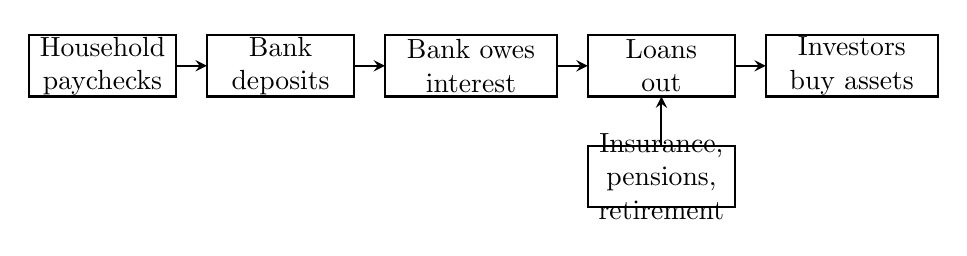
\begin{tikzpicture}[x=1cm,y=1cm,>=stealth,thick,scale=0.78]
\draw (0,0) rectangle (2.4,1) node[pos=.5,align=center]{Household\\paychecks};
\draw (2.9,0) rectangle (5.3,1) node[pos=.5,align=center]{Bank\\deposits};
\draw (5.8,0) rectangle (8.6,1) node[pos=.5,align=center]{Bank owes\\interest};
\draw (9.1,0) rectangle (11.5,1) node[pos=.5,align=center]{Loans\\out};
\draw (12.0,0) rectangle (14.8,1) node[pos=.5,align=center]{Investors\\buy assets};

\draw[->] (2.4,0.5) -- (2.9,0.5);
\draw[->] (5.3,0.5) -- (5.8,0.5);
\draw[->] (8.6,0.5) -- (9.1,0.5);
\draw[->] (11.5,0.5) -- (12.0,0.5);

\draw (9.1,-1.8) rectangle (11.5,-0.8) node[pos=.5,align=center]{Insurance,\\pensions,\\retirement};
\draw[->] (10.3,-0.8) -- (10.3,0);
\end{tikzpicture}
\end{figure}

The point is not moral outrage at finance. The point is that institutions cannot leave stored household money inert. Their own balance-sheet structure pushes the funds back into circulation, where informed borrowers can use them.

\subsection{Question \& Answer}

\paragraph{Question.} Why does saving money fail when inflation outruns the bank?

\paragraph{Answer.} McElroy's answer is a standard real-return argument stated in blunt language. If the bank pays one or two percent and inflation runs at two or three percent, purchasing power erodes.

\begin{align}
r_{\text{bank}} &\approx 1\%\text{--}2\%,\qquad \pi \approx 2\%\text{--}3\%,\\
r_{\text{real}} &\approx r_{\text{bank}} - \pi \in [-2\%,0\%].
\end{align}

This is why he says one cannot save one's way to wealth. The lecture is not claiming that liquidity is useless. It is claiming that passive nominal return below inflation is not a serious wealth strategy.

\section{Robert Kiyosaki: Debt, Sales, Rejection, and Anti-School Polemic}

\paragraph{Anecdote.} The final interview is framed as the meeting with the man who ``wrote the book on money.'' That theatrical setup matters because Kiyosaki does not merely repeat earlier lessons; he radicalizes them. Where earlier speakers imply, he states. Where earlier speakers soften, he attacks.

\paragraph{Claim.} His first move is immediate: he made his millions in real estate because real estate lets him use debt. The lecture must preserve the double claim together. Debt is power, and debt is danger.

\subsection{Question \& Answer}

\paragraph{Question.} If debt is dangerous, why does Kiyosaki still call debt money?

\paragraph{Answer.} Because debt enlarges the asset base one can control. In the barest formal reconstruction, we may write

\begin{equation}
A_{\text{acquired}} = E + D_{\text{debt}},
\end{equation}

where \(E\) is one's own equity and \(D_{\text{debt}}\) is borrowed capital. This is the positive side of the argument. But Kiyosaki immediately adds the negative side: debt is like a loaded gun. Used stupidly, it destroys the borrower. His macro illustration is political and polemical rather than academic. He cites a United States debt figure above

\begin{equation}
D_{\text{US}} > \$38\,\text{trillion}
\end{equation}

as an example of destructive misuse. The chapter should preserve the asymmetry clearly: debt is not good because it is safe; it is useful because it is dangerous and scalable.

\paragraph{Mechanism.} Kiyosaki then traces the origin of this view back to his rich-dad teaching. One must first learn to sell. His poor-dad world treated salesmen with contempt; his rich-dad world treated selling as unavoidable. Entrepreneurship, in this account, begins not with product design but with the ability to move another mind.

\subsection{Question \& Answer}

\paragraph{Question.} Why is sales treated as prior to entrepreneurship rather than downstream of it?

\paragraph{Answer.} Because Kiyosaki defines sales as communication under resistance. The real obstacle is not technique but rejection. His examples are crude, memorable, and numerically useful. He says he asked his future wife out \(50\) times, and he stayed at Xerox until he reached the top sales rank.

\begin{align}
n_{\text{asks}} &= 50,\\
\text{attempt} &\to \text{rejection} \to \text{renewed attempt}.
\end{align}

This loop is the local dynamics of his sales doctrine. Each refusal is not the end state; it is the transition rule. The same ranking ethic appears in the Xerox story:

\begin{equation}
\operatorname{rank}_{\text{Xerox}} = 1.
\end{equation}

We should not read this as a universal theorem that only the top slot matters in every domain. But within the lecture it functions as a discipline of ambition. Do not learn sales casually. Stay until you can prove to yourself that you can win.

\paragraph{Anti-school polemic.} From here the interview lands where it had been threatening to land all along: school, in Kiyosaki's telling, does not teach money. The transcript should be rendered carefully here. These are his claims, not neutral textbook statements. He says college is a scam, says school teaches nothing about money, and says he would first learn to make money before choosing a profession. Whether one agrees is secondary to the structure of the lecture. Earlier speakers complained implicitly that institutions do not teach operational finance. Kiyosaki makes the complaint explicit and attaches it to sales, debt, and ranking.

\section{Summary}

The lecture begins as a field search and ends as a compact algebra of wealth. First, wealth is concentrated but guarded, so access must be earned. Second, the move from a \$10 million firm to a \$100 million firm is really a question about prebuilt structure. Third, time is fixed at \(24\) hours, so inequality emerges through allocation. Fourth, retained capital compounds when owner draw stays small. Fifth, speed lowers response latency and keeps opportunity from decaying. Sixth, institutional money flows back out through credit markets, where informed borrowers can use it. Finally, debt, sales, and rejection are presented not as side skills but as the hard instruments of wealth building.

What makes the transcript unusually useful is that it never stays in abstraction for long. Each doctrine is tied to a person, a number, a bottleneck, a cash-flow example, or a repeated refusal. That is why the chapter should preserve the lecture's original rhythm. The host goes looking for rich people; what he gradually finds is a set of operating rules.